%%%%%%%%%%%%%%%%%%%%%%%%%%%%%%%%%%%%%%%%%%%%%%%%%%%%%%%%%%%%%%%%%%%%%%%%%%%%%%%
% PREAMBOLO COMUNE PER APPUNTI (Stile Scuro)
%
% Questo file contiene tutte le impostazioni e i pacchetti comuni.
% NON contiene \begin{document} o \end{document}.
%
% Istruzioni per la compilazione del file principale:
% pdflatex -shell-escape nomefile_principale.tex
%%%%%%%%%%%%%%%%%%%%%%%%%%%%%%%%%%%%%%%%%%%%%%%%%%%%%%%%%%%%%%%%%%%%%%%%%%%%%%%

\documentclass{article}

% --- Encoding e lingua ---
\usepackage[utf8]{inputenc}
\usepackage[italian]{babel}

% --- Margini e layout ---
\usepackage{geometry}
\geometry{a4paper, margin=1in}

% --- Font sans-serif (come Helvetica) ---
\usepackage[scaled]{helvet}
\renewcommand{\familydefault}{\sfdefault}
\usepackage[T1]{fontenc}

% --- Matematica ---
\usepackage{amsmath}
\usepackage{amssymb}

% --- Liste personalizzate ---
\usepackage{enumitem}
% \setlist{nosep}

% --- Immagini e Grafica ---
\usepackage{float}
% \usepackage{graphicx}
\usepackage{tikz}
\usetikzlibrary{shapes.geometric, positioning, arrows.meta, calc, fit, backgrounds, patterns, decorations.pathreplacing}

% --- Tabelle Avanzate ---
\usepackage{array}
\usepackage{booktabs}
\usepackage{longtable}

% --- Hyperlink e Metadati PDF ---
\usepackage{hyperref}

\hypersetup{
    colorlinks=true,
    linkcolor=white,
    filecolor=magenta,
    urlcolor=cyan,
    citecolor=green,
    % pdftitle, pdfauthor, ecc. verranno impostati nel file principale
    pdfpagemode=FullScreen,
    bookmarksopen=true,
    bookmarksnumbered=true
}

% --- Licenza del documento ---
\usepackage[
  type={CC},
  modifier={by-sa},
  version={4.0},
]{doclicense}

% --- Colori e Sfondo Nero ---
\usepackage{xcolor}
\pagecolor{black}
\color{white}

% --- Evidenziazione del Codice ---
\usepackage{minted}
\setminted{
    frame=lines,
    framesep=2mm,
    fontsize=\small,
    breaklines=true,
    style=monokai,
    bgcolor=black!80
}
\usemintedstyle{monokai}

% --- Comandi personalizzati per algebra relazionale ---
\newcommand{\Rel}[1]{\textit{#1}} % Per i nomi delle relazioni
\newcommand{\Attr}[1]{\textsf{#1}} % Per i nomi degli attributi

\newcommand{\myunion}{\cup}
\newcommand{\myintersection}{\cap}
\newcommand{\mydifference}{-}
\newcommand{\myrename}[2]{\rho_{#1}(#2)}
\newcommand{\myselectop}[2]{\sigma_{#1}(#2)}
\newcommand{\myproject}[2]{\pi_{#1}(#2)}
\newcommand{\mycartesian}{\times}
\newcommand{\mynaturaljoin}{\bowtie} % Usare \Join da amssymb se disponibile e preferito
\newcommand{\mythetajoin}[3]{#1 \bowtie_{#2} #3} % R1 \bowtie_cond R2

% --- Comandi personalizzati per logica ---
\newcommand{\mylandop}{\wedge}
\newcommand{\myvel}{\vee}
\newcommand{\mynegop}{\neg}
\newcommand{\myforallop}{\forall}
\newcommand{\myexistsop}{\exists}

% --- Join esterni (outer join) ---
% Definizione standard per i join esterni
\def\ojoin{\setbox0=\hbox{$\mynaturaljoin$}%
	\rule[-.02ex]{.25em}{.4pt}\llap{\rule[\ht0]{.25em}{.4pt}}}
\newcommand{\myleftouterjoin}{\mathbin{\ojoin\mkern-5.8mu\mynaturaljoin}}
\newcommand{\myrightouterjoin}{\mathbin{\mynaturaljoin\mkern-5.8mu\ojoin}}
\newcommand{\myfullouterjoin}{\mathbin{\ojoin\mkern-5.8mu\mynaturaljoin\mkern-5.8mu\ojoin}}



\title{Spettro Fisico, Canali Logici, Modulazione Digitale}
\author{Basato sulle slide del Prof. Luciano Bononi}
\date{\today}

\usetikzlibrary{decorations.pathmorphing}

\begin{document}

\maketitle
\tableofcontents
\newpage

\section{Spettro delle Reti Wireless e Allocazione}

\begin{itemize}
    \item \textbf{Spettro Elettromagnetico:} Le comunicazioni wireless utilizzano una porzione dello spettro elettromagnetico, principalmente le \textbf{radiofrequenze}. Questo spettro va da frequenze molto basse (udibili) a frequenze altissime (raggi Gamma).
    \item \textbf{Allocazione delle Frequenze:} Diverse tecnologie wireless operano su diverse bande di frequenza, che sono regolamentate e assegnate per evitare interferenze.
    \begin{itemize}
        \item \textbf{GSM (900/1800 MHz):} Usato per la telefonia mobile 2G.
        \item \textbf{Bluetooth, ZigBee, Wi-Fi (802.11b/g/n) a 2.4 GHz:} Questa è una banda \textbf{ISM (Industrial, Scientific, Medical)}, che è \textit{unlicensed} (non licenziata), il che significa che può essere usata liberamente da dispositivi a bassa potenza, ma è anche più soggetta a interferenze.
        \item \textbf{Wi-Fi (802.11a/ac) a 5 GHz:} Un'altra banda per Wi-Fi, spesso meno affollata della 2.4 GHz.
        \item \textbf{LMDS (Local Multipoint Distribution Service) a 28 GHz:} Usato per accessi wireless a banda larga "ultimo miglio".
        \item \textbf{IR (Infrarosso):} Usato per comunicazioni a cortissimo raggio, come i telecomandi (es. IEEE 802.11 IR).
    \end{itemize}
    \item \textbf{Fixed Spectrum Assignment:} Esiste una mappa globale (anche se con variazioni regionali) che assegna specifiche porzioni di spettro a specifici servizi (es. mobile, broadcasting, aeronautico, ecc.). Questo è fondamentale per l'organizzazione delle comunicazioni.
\end{itemize}
\begin{figure}[H]
\centering
\begin{tikzpicture}[scale=0.8, transform shape]
    % Asse delle frequenze
    \draw[->] (0,0) -- (12,0) node[right] {Frequenza (Hz)};
    
    % Labels delle frequenze
    \foreach \x/\label in {1/$10^3$, 3/$10^6$, 5/$10^9$, 7/$10^{12}$, 9/$10^{15}$, 11/$10^{18}$} {
        \draw (\x,-0.2) -- (\x,0.2);
        \node[below] at (\x,-0.2) {\small \label};
    }
    
    % Bande colorate
    \fill[red!20] (0,0.5) rectangle (2,2);    % Audio
    \fill[orange!20] (2,0.5) rectangle (4,2);  % Radio AM/FM
    \fill[yellow!20] (4,0.5) rectangle (5,2);  % Microonde
    \fill[green!20] (5,0.5) rectangle (7,2);   % IR
    \fill[blue!20] (7,0.5) rectangle (9,2);    % Visibile
    \fill[violet!20] (9,0.5) rectangle (11,2); % UV/X/Gamma
    
    % Etichette delle bande
    \node[above] at (1,2) {\small Audio};
    \node[above] at (3,2) {\small Radio};
    \node[above] at (4.5,2) {\small Microonde};
    \node[above] at (6,2) {\small IR};
    \node[above] at (8,2) {\small Visibile};
    \node[above] at (10,2) {\small UV/X/Gamma};
    
    % Punti per le tecnologie wireless
    \fill[red] (3.5,1) circle (2pt);    % GSM
    \fill[themeblue] (4.2,1) circle (2pt);   % WiFi 2.4
    \fill[themeblue] (4.4,1) circle (2pt);   % WiFi 5
    \fill[green] (4.6,1) circle (2pt);  % LMDS
    \fill[orange] (5.5,1) circle (2pt); % IR
    
    % Legenda in alto a destra
    \begin{scope}[shift={(11,2)}]
        \node[draw, rounded corners] at (2.5,0) {
            \begin{tabular}{ll}
                \textcolor{red}{$\bullet$} & GSM (900/1800 MHz) \\
                \textcolor{themeblue}{$\bullet$} & Wi-Fi 2.4 GHz \\
                \textcolor{themeblue}{$\bullet$} & Wi-Fi 5 GHz \\
                \textcolor{green}{$\bullet$} & LMDS (28 GHz) \\
                \textcolor{orange}{$\bullet$} & IR
            \end{tabular}
        };
    \end{scope}
    
    % Titolo
    \node[above] at (6,2.5) {Spettro Elettromagnetico e Allocazioni Wireless};
\end{tikzpicture}
\caption{Rappresentazione dello spettro elettromagnetico con le principali allocazioni wireless.}
\label{fig:em_spectrum}
\end{figure}

\section{Larghezza di Banda (Bandwidth) e Spettro nelle Reti Wireless}

\begin{itemize}
    \item \textbf{Come i canali wireless possono avere diversa larghezza di banda?}
    \begin{itemize}
        \item \textbf{I bit viaggiano più o meno velocemente? NO.} La velocità di propagazione è vicina a quella della luce (circa $300.000 \text{ Km/s}$) per tutti i bit.
        \item \textbf{Il "tubo" del canale (spettro) è più grande? SÌ/NO.} Avere una porzione di spettro più ampia permette di trasmettere più informazione contemporaneamente.
        \item \textbf{Il canale richiede meno tempo per accomodare (codificare) un bit sul canale? SÌ.} Tecniche di codifica più efficienti permettono di "impacchettare" più bit nello stesso intervallo di tempo o sulla stessa porzione di spettro.
    \end{itemize}
    \item \textbf{Esempio Pratico:}
    Immagina due autostrade: Canale A (1 corsia, 10 auto/ora) e Canale B (2 corsie, 20 auto/ora). Il Canale B ha una "capacità" maggiore. Nelle reti, questo si traduce in più bit/secondo.
\end{itemize}

\begin{figure}[H]
\centering
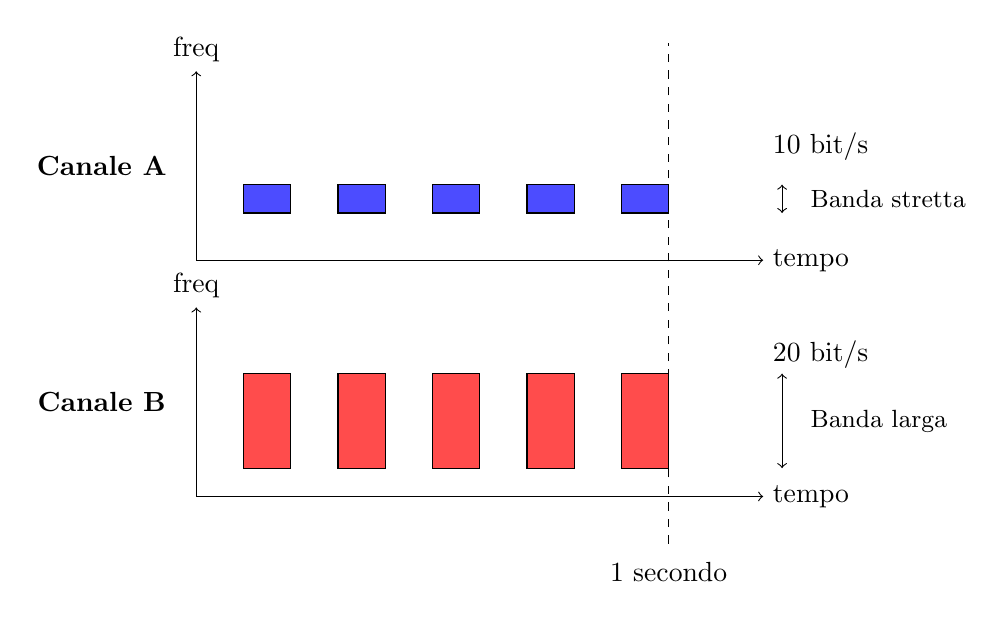
\begin{tikzpicture}[scale=1.2]
    % Canale A - Banda stretta
    \node at (-1, 4.5) {\textbf{Canale A}};
    
    % Assi per Canale A 
    \draw[->] (0,3.5) -- (0,5.5) node[above] {freq};
    \draw[->] (0,3.5) -- (6,3.5) node[right] {tempo};
    
    % Bit del Canale A (banda stretta - altezza piccola)
    \foreach \i in {0,1,2,3,4} {
        \fill[blue!70] (\i*1 + 0.5, 4) rectangle (\i*1 + 1, 4.3);
        \draw (\i*1 + 0.5, 4) rectangle (\i*1 + 1, 4.3);
    }
    
    % Indicatore larghezza banda A
    \draw[<->] (6.2, 4) -- (6.2, 4.3);
    \node[right] at (6.4, 4.15) {\small Banda stretta};
    
    \node[right] at (6, 4.7) {10 bit/s};
    
    % Canale B - Banda larga  
    \node at (-1, 2) {\textbf{Canale B}};
    
    % Assi per Canale B
    \draw[->] (0,1) -- (0,3) node[above] {freq};
    \draw[->] (0,1) -- (6,1) node[right] {tempo};
    
    % Bit del Canale B (banda larga - altezza grande)
    \foreach \i in {0,1,2,3,4} {
        \fill[red!70] (\i*1 + 0.5, 1.3) rectangle (\i*1 + 1, 2.3);
        \draw (\i*1 + 0.5, 1.3) rectangle (\i*1 + 1, 2.3);
    }
    
    % Indicatore larghezza banda B
    \draw[<->] (6.2, 1.3) -- (6.2, 2.3);
    \node[right] at (6.4, 1.8) {\small Banda larga};
    
    \node[right] at (6, 2.5) {20 bit/s};
    
    % Marcatore temporale
    \draw[dashed] (5, 0.5) -- (5, 5.8);
    \node at (5, 0.2) {1 secondo};
    
\end{tikzpicture}
\caption{Confronto larghezza di banda: il Canale B ha una banda più larga (maggiore estensione spettrale) e trasmette il doppio dei bit al secondo rispetto al Canale A.}
\label{fig:bandwidth_comparison}
\end{figure}

\section{Copertura della Trasmissione Radio}
La copertura dipende dalla potenza di trasmissione (Tx power) e dalla sensibilità del ricevitore.

\begin{figure}[H]
\centering
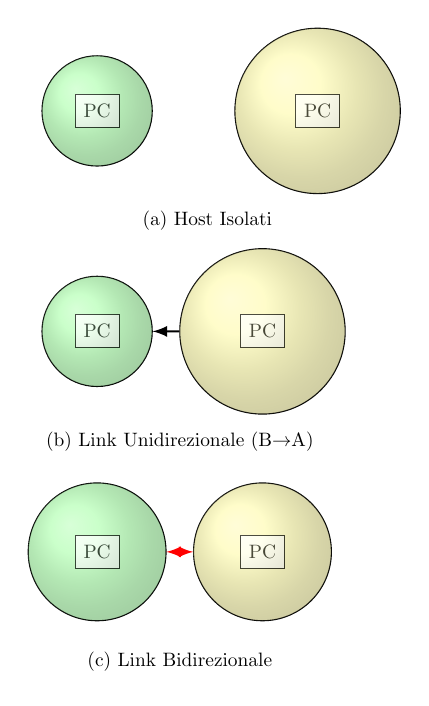
\begin{tikzpicture}[scale=0.7, transform shape]
    % Host Isolati
    \node (A1) [circle, draw, fill=green!20, minimum size=2cm, label=center:A] at (0,0) {};
    \node (PC_A1) [rectangle, draw, fill=white, minimum width=0.8cm, minimum height=0.6cm] at (A1.center) {PC};
    \shade[ball color=green!30, opacity=0.3] (A1.center) circle (1cm);

    \node (B1) [circle, draw, fill=yellow!20, minimum size=3cm, label=center:B] at (4,0) {};
    \node (PC_B1) [rectangle, draw, fill=white, minimum width=0.8cm, minimum height=0.6cm] at (B1.center) {PC};
    \shade[ball color=yellow!30, opacity=0.3] (B1.center) circle (1.5cm);
    \node at (2,-2) {(a) Host Isolati};

    % Link Unidirezionale
    \node (A2) [circle, draw, fill=green!20, minimum size=2cm, label=center:A] at (0,-4) {};
    \node (PC_A2) [rectangle, draw, fill=white, minimum width=0.8cm, minimum height=0.6cm] at (A2.center) {PC};
    \shade[ball color=green!30, opacity=0.3] (A2.center) circle (1cm);

    \node (B2) [circle, draw, fill=yellow!20, minimum size=3cm, label=center:B] at (3,-4) {};
    \node (PC_B2) [rectangle, draw, fill=white, minimum width=0.8cm, minimum height=0.6cm] at (B2.center) {PC};
    \shade[ball color=yellow!30, opacity=0.3] (B2.center) circle (1.5cm);
    \draw[-latex, thick] (B2) -- (A2);
    \node at (1.5,-6) {(b) Link Unidirezionale (B$\rightarrow$A)};

    % Link Bidirezionale
    \node (A3) [circle, draw, fill=green!20, minimum size=2.5cm, label=center:A] at (0,-8) {};
    \node (PC_A3) [rectangle, draw, fill=white, minimum width=0.8cm, minimum height=0.6cm] at (A3.center) {PC};
    \shade[ball color=green!30, opacity=0.3] (A3.center) circle (1.25cm);

    \node (B3) [circle, draw, fill=yellow!20, minimum size=2.5cm, label=center:B] at (3,-8) {};
    \node (PC_B3) [rectangle, draw, fill=white, minimum width=0.8cm, minimum height=0.6cm] at (B3.center) {PC};
    \shade[ball color=yellow!30, opacity=0.3] (B3.center) circle (1.25cm);
    \draw[latex-latex, thick, red] (A3) -- (B3);
    \node at (1.5,-10) {(c) Link Bidirezionale};
\end{tikzpicture}
\caption{Scenari di copertura radio.}
\label{fig:coverage_scenarios}
\end{figure}

\begin{itemize}
    \item \textbf{Host Isolati:} Se due dispositivi (Host A e Host B) hanno una potenza di trasmissione troppo bassa perché i loro segnali si raggiungano, sono isolati (Fig. \ref{fig:coverage_scenarios}a).
    \item \textbf{Link Unidirezionale:} Se Host B ha alta potenza e Host A bassa potenza, A potrebbe ricevere da B, ma B non riceve da A. Questo è un link unidirezionale (talvolta impropriamente detto "asimmetrico" in questo contesto) (Fig. \ref{fig:coverage_scenarios}b).
    \item \textbf{Link Bidirezionale:} Se entrambi hanno potenza sufficiente per raggiungersi a vicenda (Fig. \ref{fig:coverage_scenarios}c).
    \begin{itemize}
        \item \textbf{Link Bidirezionale Simmetrico:} La velocità di trasmissione è la stessa in entrambe le direzioni (es. A$\rightarrow$B 10Mbps, B$\rightarrow$A 10Mbps).
        \item \textbf{Link Bidirezionale Asimmetrico:} La velocità di trasmissione è diversa nelle due direzioni (es. A$\rightarrow$B 1Mbps, B$\rightarrow$A 10Mbps).
    \end{itemize}
\end{itemize}

\section{Tecnologie delle Reti Wireless}
\begin{itemize}
    \item \textbf{Narrowband Radio System (Sistema Radio a Banda Stretta):}
    \begin{itemize}
        \item Trasmette/riceve usando una singola, stretta frequenza radio, spesso licenziata.
        \item Suscettibile a cross-talk, richiede coordinamento e licenze.
        \item Tipicamente ha bassi data-rate.
        \item \textit{Esempio:} Vecchie radio walkie-talkie.
    \end{itemize}
    \item \textbf{Spread Spectrum Technology (Tecnologia a Spettro Espanso):}
    Migliora l'efficienza della larghezza di banda, l'affidabilità e la sicurezza.
    \begin{itemize}
        \item \textbf{Frequency Hopping Spread Spectrum (FHSS):}
        \begin{itemize}
            \item Il segnale a banda stretta "salta" (hops) tra diverse frequenze seguendo una sequenza pseudo-casuale nota sia al trasmettitore che al ricevitore.
            \item Per un ricevitore non sincronizzato, appare come rumore impulsivo.
            \item \textit{Esempio:} Il Bluetooth usa FHSS.
        \end{itemize}
        \begin{figure}[H]
        \centering
        \begin{tikzpicture}[scale=0.9, transform shape]
            \draw[->] (0,0) -- (6,0) node[right] {time};
            \draw[->] (0,0) -- (0,2.5) node[above] {Frequency hops};
            \foreach \y in {10,20,...,80} {
                \draw (-0.1, \y/40) node[left] {\small \y} -- (0.1, \y/40);
            }
            \draw[thick, red] (0,10/40) -- (1,10/40) -- (1,60/40) -- (2,60/40) -- (2,20/40) -- (3,20/40) -- (3,70/40) -- (4,70/40) -- (4,40/40) -- (5,40/40);
            \draw[thick, themeblue, dashed] (0,30/40) -- (0.5,30/40) -- (0.5,70/40) -- (1.5,70/40) -- (1.5,40/40) -- (2.5,40/40) -- (2.5,80/40) -- (3.5,80/40) -- (3.5,50/40) -- (4.5,50/40);
        \end{tikzpicture}
        \caption{Esempio di Frequency Hopping Spread Spectrum (FHSS).}
        \label{fig:fhss}
        \end{figure}

        \item \textbf{Direct Sequence Spread Spectrum (DSSS):}
        \begin{itemize}
            \item Ogni bit di dati viene "espanso" moltiplicandolo per una sequenza di bit più lunga (detta "chipping code"). Questo distribuisce l'energia del segnale su una banda più larga.
            \item Per un ricevitore non sincronizzato, appare come rumore a larga banda di bassa potenza.
            \item \textit{Esempio:} Wi-Fi (802.11b) e GPS usano DSSS.
        \end{itemize}
         \begin{figure}[H]
        \centering
        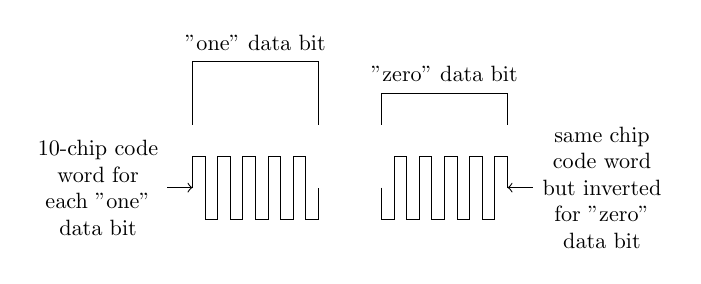
\begin{tikzpicture}[scale=0.8, transform shape]
            % "one" data bit
            \draw (0,1.5) -- (0,2.5) -- (2,2.5) -- (2,1.5);
            \node at (1,2.8) {"one" data bit};
            % 10-chip code for "one"
            \draw (0,0.5) -- (0,1) -- (0.2,1) -- (0.2,0) -- (0.4,0) -- (0.4,1) -- (0.6,1) -- (0.6,0) -- (0.8,0) -- (0.8,1) -- (1,1) -- (1,0) -- (1.2,0) -- (1.2,1) -- (1.4,1) -- (1.4,0) -- (1.6,0) -- (1.6,1) -- (1.8,1) -- (1.8,0) -- (2,0) -- (2,0.5);
            \node[text width=2cm, align=center] at (-1.5, 0.5) {10-chip code word for each "one" data bit};
            \draw[->] (-0.4,0.5) -- (0,0.5);

            % "zero" data bit
            \draw (3,1.5) -- (3,2) -- (5,2) -- (5,1.5);
            \node at (4,2.3) {"zero" data bit};
            % Inverted 10-chip code for "zero"
            \draw (3,0.5) -- (3,0) -- (3.2,0) -- (3.2,1) -- (3.4,1) -- (3.4,0) -- (3.6,0) -- (3.6,1) -- (3.8,1) -- (3.8,0) -- (4,0) -- (4,1) -- (4.2,1) -- (4.2,0) -- (4.4,0) -- (4.4,1) -- (4.6,1) -- (4.6,0) -- (4.8,0) -- (4.8,1) -- (5,1) -- (5,0.5);
            \node[text width=2cm, align=center] at (6.5, 0.5) {same chip code word but inverted for "zero" data bit};
            \draw[<-] (5,0.5) -- (5.4,0.5);
        \end{tikzpicture}
        \caption{Esempio di Direct Sequence Spread Spectrum (DSSS).}
        \label{fig:dsss_coding}
        \end{figure}
    \end{itemize}
    \item \textbf{Infrared Technology (Tecnologia Infrarossi):}
    \begin{itemize}
        \item Usa onde infrarosse. Richiede linea di vista o può essere diffusa in ambienti chiusi.
        \item \textit{Esempio:} Telecomandi TV.
    \end{itemize}
\end{itemize}

\section{Classificazione delle Reti Wireless per Copertura}
\begin{itemize}
    \item \textbf{WWAN (Wireless Wide Area Network):} Copertura geografica estesa (es. satelliti, reti cellulari).
    \item \textbf{WMAN (Wireless Metropolitan Area Network):} Copertura metropolitana (es. una città, WiMAX).
    \item \textbf{WLAN (Wireless Local Area Network):} Copertura locale (es. un edificio, una casa - Wi-Fi).
    \item \textbf{WPAN (Wireless Personal Area Network):} Copertura personale, ridotta (es. una stanza - Bluetooth).
    \item \textbf{Wireless Indoor Area Network:} Copertura a cortissimo raggio, tipicamente una stanza.
\end{itemize}

\section{Strutture delle Reti Wireless}
\subsection{WWAN e WMAN}
\begin{itemize}
    \item \textbf{Satelliti:}
    \begin{itemize}
        \item \textbf{LEO (Low Earth Orbit):} Orbita bassa.
        \item \textbf{GEO (Geostationary Orbit):} Orbita geostazionaria.
    \end{itemize}
    \item \textbf{Reti Cellulari:} Evoluzione da 1G a 5G.
    \item \textbf{Struttura Cellulare / Multi-Infrastructure WLAN:} Griglia di Access Points connessi a una Backbone.
\end{itemize}
\subsection{WLAN}
\begin{itemize}
    \item \textbf{Ad Hoc:}
    \begin{itemize}
        \item Comunicazione peer-to-peer (P2P) "al volo".
        \item Nessuna amministrazione centrale.
        \item \textit{Esempio:} Due laptop connessi direttamente via Wi-Fi.
    \end{itemize}
    \item \textbf{Infrastructure:}
    \begin{itemize}
        \item Unità di controllo centralizzata (Access Point).
        \item Roaming tra celle (AP).
        \item \textit{Esempio:} Tipica rete Wi-Fi domestica con router.
    \end{itemize}
\end{itemize}

\section{Integrazione tra Mondo Wireless e Cablato}
\begin{itemize}
    \item \textbf{Sfide:} Progettazione di protocolli wireless, integrazione, ottimizzazione (layering, bridging, Mobile IP, QoS).
    \item \textbf{Obiettivo:} Supportare applicazioni "wired-like" su dispositivi wireless.
    \item \textbf{Soluzione Possibile:}
    \begin{itemize}
        \item Scollegare reti wired e wireless per gestirle in modo indipendente ma interoperabile.
        \item Integrazione dei protocolli, mantenendo trasparenza.
        \item Strutture SW e protocolli per adattare contenuti a dispositivi eterogenei.
        \item Comportamento adattivo dei protocolli (lato wireless).
    \end{itemize}
\end{itemize}

\section{Svantaggi (Drawbacks) del Wireless}
\begin{itemize}
    \item \textbf{Capacità di Canale Ridotta:} Inferiore alle reti cablate.
    \item \textbf{Spettro Limitato:} Risorsa scarsa. Necessità di riuso.
    \item \textbf{Energia Limitata (Batterie):} Sfida per dispositivi mobili.
    \item \textbf{Rumore e Interferenza:} Impatto elevato sulle prestazioni.
    \item \textbf{Sicurezza:} Informazioni "on the air", intercettabili.
    \item \textbf{Gestione della Mobilità:} Indirizzamento e routing (es. Mobile IP).
    \item \textbf{Tracciamento della Posizione (Location Tracking):} Paging, LBS.
    \item \textbf{Gestione della QoS (Quality of Service):} Complessa, multi-livello.
    \item \textbf{Servizi Best Effort:} Servizio base senza garanzie.
\end{itemize}

\section{Canale Logico Wireless e Multiplexing}
Il \textbf{multiplexing} permette a più utenti/segnali di condividere lo stesso mezzo trasmissivo.
\begin{itemize}
    \item \textbf{Dimensioni del Multiplexing:} Spazio ($s_i$), Tempo (t), Frequenza (f), Codice (c).
    \item \textbf{Importante:} Necessari "spazi di guardia" (guard spaces) per evitare interferenze.
\end{itemize}

\begin{figure}[H]
\centering
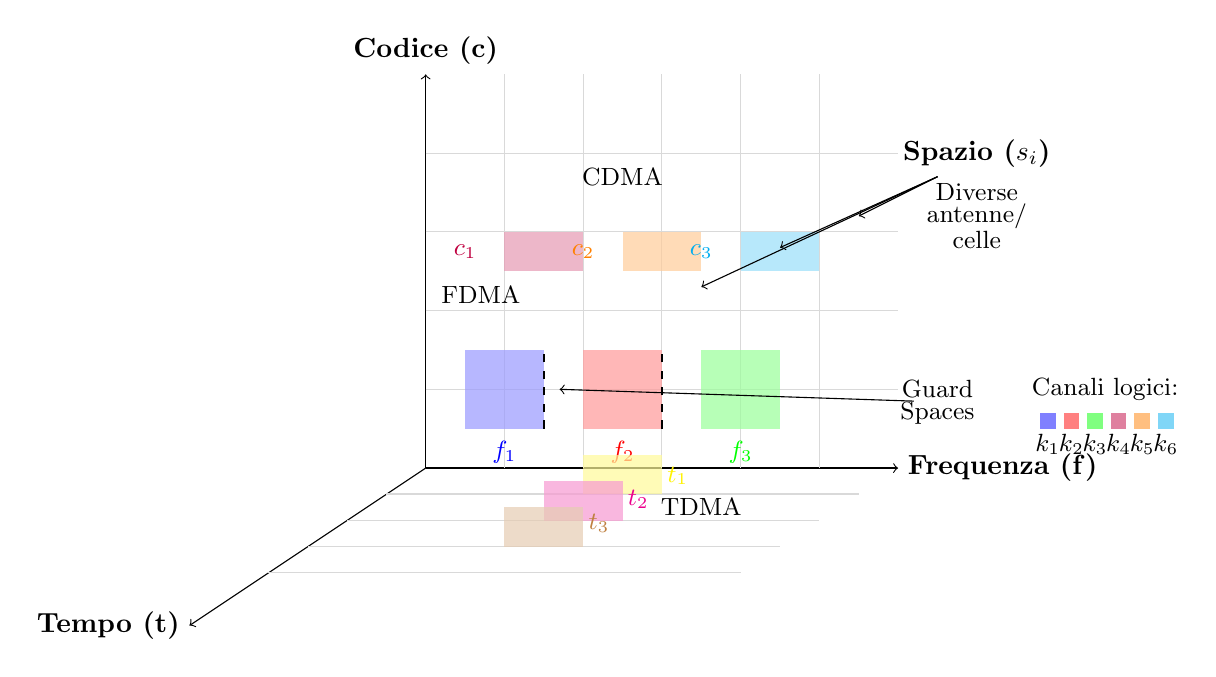
\begin{tikzpicture}[transform shape]
    % Main 3D coordinate system
    \draw[->] (0,0) -- (6,0) node[right] {\textbf{Frequenza (f)}};
    \draw[->] (0,0) -- (0,5) node[above] {\textbf{Codice (c)}};
    \draw[->] (0,0) -- (-3,-2) node[left] {\textbf{Tempo (t)}};
    
    % Grid lines to show 3D space
    \draw[gray!30] (1,0) -- (1,5);
    \draw[gray!30] (2,0) -- (2,5);
    \draw[gray!30] (3,0) -- (3,5);
    \draw[gray!30] (4,0) -- (4,5);
    \draw[gray!30] (5,0) -- (5,5);
    
    \draw[gray!30] (0,1) -- (6,1);
    \draw[gray!30] (0,2) -- (6,2);
    \draw[gray!30] (0,3) -- (6,3);
    \draw[gray!30] (0,4) -- (6,4);
    
    % Time dimension grid (3D effect)
    \draw[gray!30] (-0.5,-0.33) -- (5.5,-0.33);
    \draw[gray!30] (-1,-0.67) -- (5,-0.67);
    \draw[gray!30] (-1.5,-1) -- (4.5,-1);
    \draw[gray!30] (-2,-1.33) -- (4,-1.33);
    
    % Different channels represented as colored rectangles in different dimensions
    
    % FDMA - Frequency Division (different frequency bands)
    \fill[blue!40, opacity=0.7] (0.5,0.5) rectangle (1.5,1.5);
    \fill[red!40, opacity=0.7] (2,0.5) rectangle (3,1.5);
    \fill[green!40, opacity=0.7] (3.5,0.5) rectangle (4.5,1.5);
    \node at (0.7,2.2) {\small FDMA};
    \node[blue] at (1,0.2) {\small $f_1$};
    \node[red] at (2.5,0.2) {\small $f_2$};
    \node[green] at (4,0.2) {\small $f_3$};
    
    % CDMA - Code Division (different code sequences)
    \fill[purple!40, opacity=0.7] (1,2.5) rectangle (2,3);
    \fill[orange!40, opacity=0.7] (2.5,2.5) rectangle (3.5,3);
    \fill[cyan!40, opacity=0.7] (4,2.5) rectangle (5,3);
    \node at (2.5,3.7) {\small CDMA};
    \node[purple] at (0.5,2.75) {\small $c_1$};
    \node[orange] at (2,2.75) {\small $c_2$};
    \node[cyan] at (3.5,2.75) {\small $c_3$};
    
    % TDMA - Time Division (3D perspective showing time slots)
    \fill[yellow!40, opacity=0.7] (2,-0.33) rectangle (3,0.17);
    \fill[magenta!40, opacity=0.7] (1.5,-0.67) rectangle (2.5,-0.17);
    \fill[brown!40, opacity=0.7] (1,-1) rectangle (2,-0.5);
    \node at (3.5,-0.5) {\small TDMA};
    \node[yellow] at (3.2,-0.1) {\small $t_1$};
    \node[magenta] at (2.7,-0.4) {\small $t_2$};
    \node[brown] at (2.2,-0.7) {\small $t_3$};
    
    % Guard spaces illustration
    \draw[dashed, thick] (1.5,0.5) -- (1.5,1.5);
    \draw[dashed, thick] (3,0.5) -- (3,1.5);
    \node at (6.5,1) {\small Guard};
    \node at (6.5,0.7) {\small Spaces};
    \draw[->] (6.2,0.85) -- (1.7,1);
    
    % Spatial dimension indication
    \node at (7,4) {\textbf{Spazio ($s_i$)}};
    \draw[->] (6.5,3.7) -- (5.5,3.2);
    \draw[->] (6.5,3.7) -- (4.5,2.8);
    \draw[->] (6.5,3.7) -- (3.5,2.3);
    \node at (7,3.5) {\small Diverse};
    \node at (7,3.2) {\small antenne/};
    \node at (7,2.9) {\small celle};
    
    % Legend
    \node at (8.63,1) {\small Canali logici:};
    \foreach \i/\col in {1/blue,2/red,3/green,4/purple,5/orange,6/cyan}{
        \fill[\col!50] (7.5+\i*0.3, 0.5) rectangle (7.7+\i*0.3, 0.7);
        \node at (7.6+\i*0.3, 0.3) {\small $k_{\i}$};
    }
\end{tikzpicture}
\caption{Dimensioni del multiplexing: separazione dei canali mediante Frequenza (FDMA), Tempo (TDMA), Codice (CDMA) e Spazio (SDMA). Gli spazi di guardia prevengono le interferenze tra canali adiacenti.}
\label{fig:multiplex_dimensions}
\end{figure}

\subsection{Frequency Multiplex (FDM)}
\begin{itemize}
    \item L'intero spettro è diviso in bande di frequenza più piccole. Ogni canale ottiene una banda per tutto il tempo.
    \item \textbf{Vantaggi:} No coordinazione dinamica, funziona per segnali analogici.
    \item \textbf{Svantaggi:} Spreco di banda, inflessibile, spazi di guardia.
    \item \textit{Esempio:} Stazioni radio FM.
\end{itemize}
\begin{figure}[H]
    \centering
    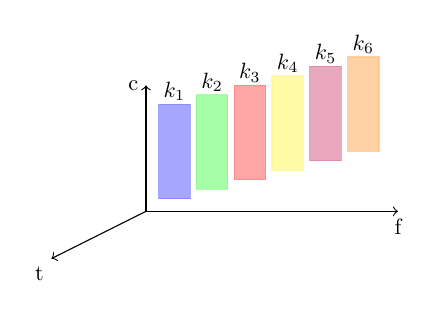
\begin{tikzpicture}[scale=0.8, transform shape]
        \draw[->] (0,0) -- (0,2) node[left]{c};
        \draw[->] (0,0) -- (4,0) node[below]{f};
        \draw[->] (0,0) -- (-1.5,-0.75) node[below left]{t};

        \foreach \i/\col in {0/blue,1/green,2/red,3/yellow,4/purple,5/orange}{
          \pgfmathsetmacro{\xshift}{\i*0.6}
          \pgfmathsetmacro{\yshift}{\i*0.5*0.3}
          \filldraw[\col!50, opacity=0.7]
            ([xshift=\xshift cm, yshift=\yshift cm]0.2,0.2)
            rectangle ++(0.5, 1.5);
          % Label aligned slightly above the top of each rectangle
          \node at (0.45+\xshift, 1.9+\yshift) {$k_{\the\numexpr\i+1\relax}$};
        }
    \end{tikzpicture}
    \caption{Frequency Division Multiplexing (FDM).}
    \label{fig:fdm}
\end{figure}


\subsection{Time Multiplex (TDM)}
\begin{itemize}
    \item Un canale ottiene l'intero spettro per un certo periodo di tempo (time slot).
    \item \textbf{Vantaggi:} Solo un carrier alla volta, throughput elevato.
    \item \textbf{Svantaggi:} Precisa sincronizzazione necessaria.
    \item \textit{Esempio:} Slot di tempo in GSM.
\end{itemize}
\begin{figure}[H]
    \centering
    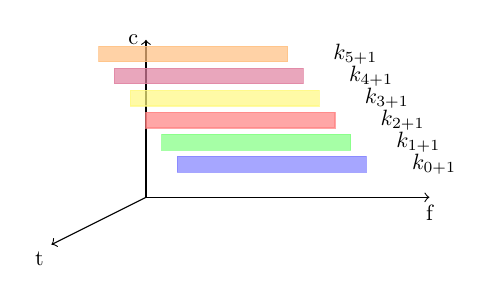
\begin{tikzpicture}[scale=0.8, transform shape]
        % Assi
        \draw[->] (0,0) -- (0,2.5) node[left]{c};
        \draw[->] (0,0) -- (4.5,0) node[below]{f};
        \draw[->] (0,0) -- (-1.5,-0.75) node[below left]{t};
        
        % Slot colorati + label
        \foreach \i/\col in {0/blue,1/green,2/red,3/yellow,4/purple,5/orange}{
            % Calcolo coordinata y
            \pgfmathsetmacro{\y}{0.4 + \i*0.3}
            % Rettangolo
            \filldraw[\col!50, opacity=0.7] 
                ([xshift=-\i*0.25cm, yshift=\i*0.05cm]0.5, \y) 
                rectangle 
                ([xshift=-\i*0.25cm, yshift=\i*0.05cm]3.5, \y + 0.25);
            % Label allineata verticalmente al centro del rettangolo
            \node[right] at ([xshift=3.6cm - \i*0.25cm, yshift=\i*0.05cm]0.5, \y + 0.125) {$k_{\i+1}$};
        }
    \end{tikzpicture}
    \caption{Time Division Multiplexing (TDM).}
    \label{fig:tdm}
\end{figure}
\begin{figure}[H]
    \centering
    \includegraphics[width=0.8\linewidth]{images/tdm_multiplexing.png}
    \caption{Vista del TDM in 3D.}
    \label{fig:tdm_3d}
\end{figure}


\subsection{Time and Frequency Multiplex}
\begin{itemize}
    \item Combinazione: un canale ottiene una banda di frequenza per un periodo di tempo.
    \item \textit{Esempio:} GSM.
    \item \textbf{Vantaggi:} Migliore protezione, data rate più alti.
    \item \textbf{Svantaggi:} Precisa coordinazione.
\end{itemize}
\begin{figure}[H]
    \centering
    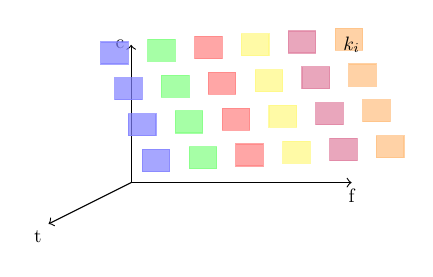
\begin{tikzpicture}[scale=0.7, transform shape]
        \draw[->] (0,0) -- (0,2.5) node[left]{c};
        \draw[->] (0,0) -- (4,0) node[below]{f};
        \draw[->] (0,0) -- (-1.5,-0.75) node[below left]{t};
         \foreach \row in {0,...,3}{
            \foreach \colidx/\col in {0/blue,1/green,2/red,3/yellow,4/purple,5/orange}{
               \filldraw[\col!50, opacity=0.7] % Use filldraw
                ([xshift=-0.25*\row cm + \colidx*0.5*0.5cm, yshift=\row*0.5*0.3cm + \colidx*0.5*0.1cm]0.2+\colidx*0.6, 0.2+\row*0.5) rectangle ([xshift=-0.25*\row cm + \colidx*0.5*0.5cm, yshift=\row*0.5*0.3cm + \colidx*0.5*0.1cm]0.2+\colidx*0.6+0.5, 0.2+\row*0.5+0.4);
            }
         }
         \node at (4,2.5) {$k_i$};
    \end{tikzpicture}
    \caption{Time and Frequency Multiplex.}
    \label{fig:tdm_fdm}
\end{figure}
\begin{figure}[H]
    \centering
    \includegraphics[width=0.8\linewidth]{images/tfdm_multiplexing.png}
    \caption{Vista del Time and Frequency Multiplex in 3D.}
    \label{fig:tfdm_3d}
\end{figure}


\subsection{Code Multiplex (CDM / CDMA)}
\begin{itemize}
    \item Ogni canale ha un codice univoco. Tutti usano lo stesso spettro nello stesso momento.
    \item \textbf{Vantaggi:} Efficienza di banda, no coordinazione stretta, buona protezione.
    \item \textbf{Svantaggi:} Data rate utente più bassi, rigenerazione complessa.
    \item Implementato con spread spectrum. \textit{Esempio:} Reti 3G.
\end{itemize}

\section{Pianificazione delle Frequenze}
\begin{itemize}
    \item \textbf{Riuso delle Frequenze:} Le stesse frequenze possono essere riutilizzate in celle non adiacenti.
    \item \textbf{Modello Standard a 7 Frequenze:} Pattern comune per allocare frequenze.
    \item \textbf{Assegnazione Fissa vs. Dinamica.}
\end{itemize}
\begin{figure}[H]
\centering
\begin{tikzpicture}[scale=0.8, transform shape,
    hexagon/.style={regular polygon, regular polygon sides=6, minimum size=1.5cm, draw, thick}]
    \node[hexagon, label=center:$f_1$] (c1) {};
    \node[hexagon, label=center:$f_2$, right=0.01cm of c1, anchor=west, xshift=-0.38cm, yshift=0.65cm] (c2) {};
    \node[hexagon, label=center:$f_3$, right=0.01cm of c2, anchor=west, xshift=-0.38cm, yshift=0.65cm] (c3) {};
    \node[hexagon, label=center:$f_4$, right=0.01cm of c1, anchor=west, xshift=-0.38cm, yshift=-0.65cm] (c4) {};
    \node[hexagon, label=center:$f_5$, right=0.01cm of c4, anchor=west, xshift=-0.38cm, yshift=-0.65cm] (c5) {};
    \node[hexagon, label=center:$f_6$, left=0.01cm of c1, anchor=east, xshift=0.38cm, yshift=0.65cm] (c6) {};
    \node[hexagon, label=center:$f_7$, left=0.01cm of c1, anchor=east, xshift=0.38cm, yshift=-0.65cm] (c7) {};
\end{tikzpicture}
\caption{Cluster di 7 celle per il riuso delle frequenze.}
\label{fig:frequency_planning}
\end{figure}

\section{Modulazione}
Processo di variare proprietà di un segnale portante con un segnale modulante.
\begin{itemize}
    \item \textbf{Modulazione Digitale:} Dati digitali $\rightarrow$ segnale analogico (baseband).
    \begin{itemize}
        \item \textbf{ASK (Amplitude Shift Keying)}
        \item \textbf{FSK (Frequency Shift Keying)}
        \item \textbf{PSK (Phase Shift Keying)}
    \end{itemize}
    \item \textbf{Modulazione Analogica (su portante RF):} Sposta il segnale baseband sulla portante radio.
    \item \textbf{Motivazione:} Antenne più piccole, FDM, caratteristiche del mezzo.
    \item \textbf{Schemi Base (per portante RF):} AM, FM, PM.
\end{itemize}


\subsection{Processo di Trasmissione di Bit con Onde Radio}
\begin{figure}[H]
\centering
\begin{tikzpicture}[node distance=1.5cm, auto,
    block/.style={rectangle, draw, fill=blue!20, text=black, text width=7em, text centered, rounded corners, minimum height=2em},
    line/.style={draw, -latex},
    wave/.style={draw, -latex, decorate, decoration={snake}}]

    \node [text width=6em] (info_in) {Info Digitale 101101001};
    \node [block, right=of info_in] (dig_mod) {Modulazione Digitale};
    \node [block, right=2.5cm of dig_mod] (ana_mod) {Modulazione Analogica};
    \node [text width=6em, right=of ana_mod] (radio_out) {Emissione Radio (segnale RF)};
    \node [coordinate, below=0.5cm of dig_mod] (baseband_mid) {};
    \node [coordinate, below=0.5cm of ana_mod] (carrier_mid) {};

    \draw [line] (info_in) -- (dig_mod);
    \draw [line, dashed] (dig_mod.east) -- node[midway,above,yshift=0.1cm] {\small Analog (baseband)} (ana_mod.west);
    \draw [line, dashed] (ana_mod.south) ++(0,-0.1) -- node[midway,right,xshift=0.1cm] {\small Carrier} (carrier_mid);
    \draw [line, dashed] (ana_mod.east) -- (radio_out.west);

    % Ricezione
    \node [text width=6em, below=3cm of radio_out] (radio_in) {Segnale RF ricevuto};
    \node [block, left=of radio_in] (ana_demod) {Demod. Analogica};
    \node [block, left=2.5cm of ana_demod] (dig_demod) {Interpret. (Demod. Digit.)};
    \node [text width=6em, left=of dig_demod] (info_out) {Info Digitale (es. 101111000)};
    \node [coordinate, below=0.5cm of ana_demod] (carrier_mid_rx) {};
    \node [coordinate, below=0.5cm of dig_demod] (baseband_mid_rx) {};

    \draw [line] (radio_in.west) -- (ana_demod.east);
    \draw [line, dashed] (ana_demod.south) ++(0,-0.1) -- node[midway,right,xshift=0.1cm] {\small Carrier} (carrier_mid_rx);
    \draw [line, dashed] (ana_demod.west) -- node[midway,above,yshift=0.1cm] {\small Analog (baseband)} (dig_demod.east);
    \draw [line] (dig_demod.west) -- (info_out.east);

    % Canale con problemi
    \path (radio_out.south) edge[line, bend right=20, dashed, red] node[midway, below, yshift=0.5cm, text width=9em] {Canale (Rumore, Interferenze)} (radio_in.north);

\end{tikzpicture}
\caption{Processo di modulazione e demodulazione.}
\label{fig:mod_demod_process}
\end{figure}

\section{Tecniche di Modulazione Digitale (Shift Keying)}
\begin{figure}[H]
\centering
\begin{tikzpicture}[scale=0.7, transform shape]
    \draw[->] (-0.5,0) -- (5.5,0) node[right]{t};
    \draw (-0.2,-1.2) -- (-0.2,1.2);
    % ASK
    \node at (-1, 2.5) {ASK};
    \draw[dashed] (0,2) -- (1,2) (1,2.8) -- (2,2.8) -- (2,1.2) -- (3,1.2) (3,2.8) -- (4,2.8) -- (4,1.2) -- (5,1.2); % Bits 0 1 0 1
    \draw[themeblue, domain=1:2, samples=20, variable=\x] plot (\x, {0.8*sin(5*(\x-1) r) + 2}); % 1
    \draw[themeblue] (0,2) -- (1,2); % 0
    \draw[themeblue, domain=3:4, samples=20, variable=\x] plot (\x, {0.8*sin(5*(\x-3) r) + 2}); % 1
    \draw[themeblue] (2,2) -- (3,2); % 0
    \node at (0.5,3) {0}; \node at (1.5,3) {1}; \node at (2.5,3) {0}; \node at (3.5,3) {1};

    % FSK
    \node at (-1, -0.5) {FSK};
    \draw[dashed] (0,-1) -- (1,-1) (1, -0.2) -- (2,-0.2) -- (2,-1.8) -- (3,-1.8) (3,-0.2) -- (4,-0.2) -- (4,-1.8) -- (5,-1.8);
    \draw[green!50!black, domain=0:1, samples=20, variable=\x] plot (\x, {0.4*sin(10*\x r) -1}); % Low freq for 0
    \draw[green!50!black, domain=1:2, samples=20, variable=\x] plot (\x, {0.4*sin(20*(\x-1) r) -1}); % High freq for 1
    \draw[green!50!black, domain=2:3, samples=20, variable=\x] plot (\x, {0.4*sin(10*(\x-2) r) -1}); % Low freq for 0
    \draw[green!50!black, domain=3:4, samples=20, variable=\x] plot (\x, {0.4*sin(20*(\x-3) r) -1}); % High freq for 1
    \node at (0.5,0) {0}; \node at (1.5,0) {1}; \node at (2.5,0) {0}; \node at (3.5,0) {1};

    % PSK
    \node at (-1, -3.5) {PSK};
    \draw[dashed] (0,-3) -- (1,-3) (1,-2.2) -- (2,-2.2) (2,-3.8) -- (3,-3.8) (3,-2.2) -- (4,-2.2);
    \draw[red, domain=0:1, samples=20, variable=\x] plot (\x, {0.8*sin(5*\x r) -3}); % Phase 0 for 0
    \draw[red, domain=1:2, samples=20, variable=\x] plot (\x, {0.8*sin(5*(\x-1) r + pi r) -3}); % Phase pi for 1
    \draw[red, domain=2:3, samples=20, variable=\x] plot (\x, {0.8*sin(5*(\x-2) r) -3}); % Phase 0 for 0
    \draw[red, domain=3:4, samples=20, variable=\x] plot (\x, {0.8*sin(5*(\x-3) r + pi r) -3}); % Phase pi for 1
    \node at (0.5,-2) {0}; \node at (1.5,-2) {1}; \node at (2.5,-2) {0}; \node at (3.5,-2) {1};
\end{tikzpicture}
\caption{Tecniche di Shift Keying: ASK, FSK, PSK.}
\label{fig:shift_keying}
\end{figure}
\begin{itemize}
    \item \textbf{ASK:} Semplice (ON/OFF), poche risorse di spettro, suscettibile a interferenze.
    \item \textbf{FSK:} Usa più spettro, due frequenze per '1' e '0', più robusta di ASK.
    \item \textbf{PSK:} Più complessa, più robusta, varia la fase della portante.
\end{itemize}

\begin{figure}[H]
\centering
\includegraphics[width=0.8\linewidth]{images/modulation_comparison.png}
\caption{Confronto tra tecniche di modulazione: ASK, FSK, PSK.}
\label{fig:modulation_comparison}
\end{figure}

\section{Rappresentazione del Segnale}
\begin{itemize}
    \item \textbf{Dominio dell'Ampiezza:} Amiezza (V) vs Tempo (s).
    \item \textbf{Dominio della Frequenza:} Ampiezza vs Frequenza (Hz).
    \item \textbf{Diagramma di Fase e Ampiezza (Diagramma di Costellazione / IQ):}
    Rappresenta ampiezza (M) e fase ($\phi$) in coordinate polari. Asse I (In-phase): $M \cos \phi$, Asse Q (Quadrature): $M \sin \phi$. Ogni \textbf{SIMBOLO} è un punto.
\end{itemize}
\begin{figure}[H]
\centering
\begin{tikzpicture}[scale=0.8, transform shape]
    \draw[->] (-1.5,0) -- (1.5,0) node[right] {I ($M \cos \phi$)};
    \draw[->] (0,-1.5) -- (0,1.5) node[above] {Q ($M \sin \phi$)};
    \coordinate (O) at (0,0);
    \coordinate (P) at (45:1); % Esempio: M=1, phi=45 deg
    \draw[thick, themeblue, ->] (O) -- (P) node[midway, above right, black] {simbolo};
    \draw (O) -- (0.3,0) arc (0:45:0.3);
    \node at (22.5:0.5) {$\phi$};
    \fill (P) circle (2pt);
\end{tikzpicture}
\caption{Diagramma di Costellazione (IQ).}
\label{fig:iq_diagram}
\end{figure}

\section{Esempi di Modulazione PSK e QAM}
\subsection{BPSK (Binary Phase Shift Keying)}
\begin{itemize}
    \item Ogni simbolo = 1 bit. Bit 0: fase 0°; Bit 1: fase 180°.
    \item Semplice, robusta. Bassa efficienza spettrale.
\end{itemize}
\begin{figure}[H] \centering
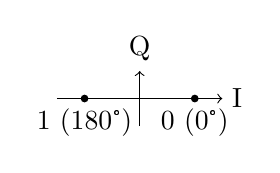
\begin{tikzpicture}[scale=0.7]
    \draw[->] (-1.5,0) -- (1.5,0) node[right] {I}; \draw[->] (0,-0.5) -- (0,0.5) node[above] {Q};
    \fill (1,0) circle (2pt) node[below] {0 (0°)}; \fill (-1,0) circle (2pt) node[below] {1 (180°)};
\end{tikzpicture}
\caption{BPSK IQ Diagram.}
\end{figure}

\subsection{QPSK (Quadrature Phase Shift Keying)}
\begin{itemize}
    \item Ogni simbolo = 2 bit (es. 00: +45°, 01: +135°, 10: +225°, 11: +315°).
    \item Più complessa e vulnerabile, ma doppia efficienza spettrale.
\end{itemize}
\begin{figure}[H] \centering
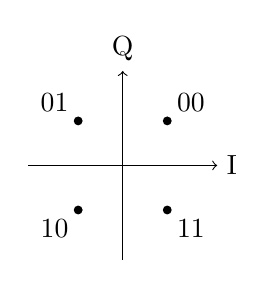
\begin{tikzpicture}[scale=0.8]
    \draw[->] (-1.5,0) -- (1.5,0) node[right] {I}; \draw[->] (0,-1.5) -- (0,1.5) node[above] {Q};
    \fill (0.707,0.707) circle (2pt) node[above right] {00}; % 45
    \fill (-0.707,0.707) circle (2pt) node[above left] {01};  % 135
    \fill (-0.707,-0.707) circle (2pt) node[below left] {10}; % 225
    \fill (0.707,-0.707) circle (2pt) node[below right] {11}; % 315
\end{tikzpicture} \caption{QPSK IQ Diagram.} \end{figure}

\subsection{Analogia "Tiro al Bersaglio" e Area del Bersaglio}
\begin{itemize}
    \item Il trasmettitore "lancia" simboli. Il ricevitore interpreta il simbolo "più vicino".
    \item \textbf{Canale Rumoroso:} Si usa BPSK (bersagli grandi/lontani).
    \item \textbf{Canale Buono:} Si usa QPSK/QAM (più bit/simbolo, bersagli più piccoli/vicini).
\end{itemize}

\subsection{Associazione Bit-Simboli (Gray Coding)}
\begin{itemize}
    \item \textbf{Gray Coding:} Simboli adiacenti nel diagramma IQ differiscono per un solo bit.
    \item Minimizza gli errori di bit: se un simbolo è confuso con uno adiacente, solo 1 bit è errato.
\end{itemize}
\begin{figure}[H] \centering
\begin{tikzpicture}[scale=0.8]
    \node at (-2.5,0) {A) No Gray};
    \draw[->] (-1.5,0) -- (1.5,0) node[right] {I}; \draw[->] (0,-1.5) -- (0,1.5) node[above] {Q};
    \fill (0.707,0.707) circle (2pt) node[above right] {00};
    \fill (-0.707,0.707) circle (2pt) node[above left] {01};
    \fill (-0.707,-0.707) circle (2pt) node[below left] {11}; % Errore di 2 bit se da 00
    \fill (0.707,-0.707) circle (2pt) node[below right] {10};
    \draw[red, thick, dashed, ->] (0.707,0.707) -- (-0.707,-0.707) node[midway, fill=white, text=red] {Errore 2 bit!};

    \node at (4.5,0) {B) Gray Coding};
    \begin{scope}[xshift=6cm]
    \draw[->] (-1.5,0) -- (1.5,0) node[right] {I}; \draw[->] (0,-1.5) -- (0,1.5) node[above] {Q};
    \fill (0.707,0.707) circle (2pt) node[above right] {00};
    \fill (-0.707,0.707) circle (2pt) node[above left] {01};
    \fill (-0.707,-0.707) circle (2pt) node[below left] {11}; % Gray coded
    \fill (0.707,-0.707) circle (2pt) node[below right] {10}; % Gray coded
    \draw[themeblue, thick, dashed, ->] (0.707,0.707) -- (0.707,-0.707) node[midway, fill=white, text=themeblue] {Errore 1 bit};
    \end{scope}
\end{tikzpicture} \caption{Confronto Gray Coding (NB: etichette simboli semplificate).} \end{figure}

\subsection{Rilevamento e Correzione Errori}
\begin{itemize}
    \item \textbf{Bit di Parità:} Rileva errori singoli.
    \item \textbf{Matrice di Bit di Parità:} Permette di identificare e correggere un singolo bit errato.
\end{itemize}

\subsection{QAM (Quadrature Amplitude Modulation)}
\begin{itemize}
    \item Combina modulazione di ampiezza E di fase. $2^n$ simboli, $n$ bit/simbolo.
    \item \textbf{16-QAM:} 16 simboli, 4 bit/simbolo.
    \item Area del "bersaglio" si riduce con $n$, più sensibile al rumore ma più efficiente.
\end{itemize}
\begin{figure}[H] \centering
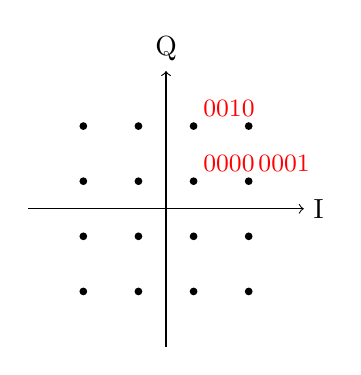
\begin{tikzpicture}[scale=0.7]
    \draw[->] (-2.5,0) -- (2.5,0) node[right] {I}; \draw[->] (0,-2.5) -- (0,2.5) node[above] {Q};
    \foreach \x in {-1.5, -0.5, 0.5, 1.5} {
        \foreach \y in {-1.5, -0.5, 0.5, 1.5} {
            \fill (\x,\y) circle (2pt);
        }
    }
    \node at (0.5,0.5) [above right, font=\small, red] {0000}; % Esempio
    \node at (1.5,0.5) [above right, font=\small, red] {0001}; % Esempio
    \node at (0.5,1.5) [above right, font=\small, red] {0010}; % Esempio
\end{tikzpicture} \caption{16-QAM IQ Diagram (16 simboli).} \end{figure}

\subsection{Modulazione Gerarchica}
\begin{itemize}
    \item Modula due sequenze di bit con priorità diverse.
    \item \textbf{Esempio 64-QAM Gerarchica (Videochiamata):}
    \begin{itemize}
        \item 6 bit/simbolo. Diagramma IQ diviso in 4 "gray clouds" (quadranti).
        \item 4 bit (bassa priorità, video) per i sotto-simboli nella cloud.
        \item 2 bit (alta priorità, voce) per etichettare la cloud.
        \item \textbf{Basso Rumore:} Voce e video OK.
        \item \textbf{Alto Rumore:} Errori video, ma voce preservata (cloud corretta identificata).
    \end{itemize}
\end{itemize}

\section{Tecniche Avanzate di Trasmissione e Accesso Multiplo}
\subsection{Spreading e Fading Selettivo in Frequenza}
\begin{itemize}
    \item Il \textit{fading} è un'attenuazione del segnale dipendente dalla frequenza.
    \item Lo \textit{spread spectrum} distribuisce l'energia su una banda più ampia, rendendo il segnale più robusto.
\end{itemize}

\subsection{DSSS (Direct Sequence Spread Spectrum) - Dettagli}
\begin{itemize}
    \item XOR del segnale dati con una \textit{chipping sequence}.
    \item Molti "chip" per bit $\rightarrow$ maggiore larghezza di banda.
    \item \textbf{Assegnazione Canali IEEE 802.11b (DSSS):} Canali non sovrapposti (es. 1, 6, 11) per evitare interferenze.
\end{itemize}
\begin{figure}[H]
\centering
\begin{tikzpicture}[yscale=0.6,xscale=0.5]
    \draw[->] (0,0) -- (15,0) node[below right] {Frequency (GHz)};
    \draw[->] (0,0) -- (0,3) node[left] {Power};
    \node[below, font=\small] at (2.5,0) {2.412 (Ch1)};
    \node[below, font=\small] at (7.5,0) {2.437 (Ch6)};
    \node[below, font=\small] at (12.5,0) {2.462 (Ch11)};
    \foreach \center/\col in {2.5/red, 7.5/green, 12.5/themeblue}{
        \fill[\col!30] (\center-2,0) rectangle (\center+2,1); % Sidelobes
        \fill[\col!70] (\center-1,0) rectangle (\center+1,2.5); % Mainlobe
        \draw (\center-2,0) -- (\center-2,1) -- (\center-1,1) -- (\center-1,2.5) -- (\center+1,2.5) -- (\center+1,1) -- (\center+2,1) -- (\center+2,0);
    }
    \node at (7.5, 3.5) {Canali DSSS non sovrapposti (es. 1, 6, 11)};
\end{tikzpicture}
\caption{Esempio di canali DSSS non sovrapposti in IEEE 802.11b.}
\label{fig:dsss_channels}
\end{figure}

\subsection{CDMA (Code Division Multiple Access) - Dettagli}
\begin{itemize}
    \item Usa DSSS. Ogni utente ha un codice univoco.
    \item Tutti trasmettono sulla stessa frequenza contemporaneamente.
    \item Il ricevitore usa il codice per estrarre il segnale desiderato.
\end{itemize}

\begin{figure}[H]
    \centering
    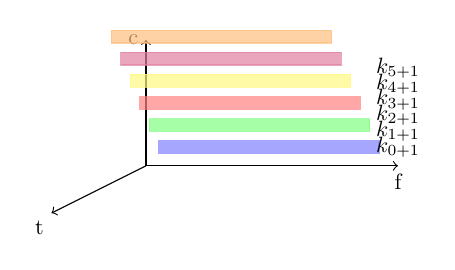
\begin{tikzpicture}[scale=0.8, transform shape]
        \draw[->] (0,0) -- (0,2) node[left]{c};
        \draw[->] (0,0) -- (4,0) node[below]{f};
        \draw[->] (0,0) -- (-1.5,-0.75) node[below left]{t};
         \foreach \i/\col in {0/blue,1/green,2/red,3/yellow,4/purple,5/orange}{
          \filldraw[\col!50, opacity=0.7] % Use filldraw
            ([xshift=-\i*0.15cm, yshift=\i*0.1cm]0.2, 0.2+\i*0.25) rectangle ([xshift=-\i*0.15cm, yshift=\i*0.1cm]0.2+3.5, 0.2+\i*0.25+0.2);
          \node at (4, 0.3+\i*0.25) {$k_{\i+1}$};
        }
    \end{tikzpicture}
    \caption{Code Division Multiplexing (CDM).}
    \label{fig:cdm}
\end{figure}
\begin{figure}[H]
    \centering
    \includegraphics[width=0.9\linewidth]{images/cdma_multiplexing.png}
    \caption{Vista del Code Division Multiplex in 3D.}
    \label{fig:cdm_3d}
\end{figure}

\subsection{FHSS (Frequency Hopping Spread Spectrum) - Dettagli}
\begin{itemize}
    \item Cambiamenti discreti della frequenza portante.
    \item \textbf{Fast Hopping:} Diverse frequenze/bit. \textbf{Slow Hopping:} Diversi bit/frequenza.
\end{itemize}

\subsection{OFDM (Orthogonal Frequency Division Multiplexing)}
\begin{itemize}
    \item Trasmette dati su molte \textbf{sottoportanti (subcarriers)} parallele ortogonali.
    \item \textbf{Vantaggi:} Alta efficienza spettrale, robustezza al multipath fading.
    \item \textbf{Funzionamento (semplificato):} Flusso bit diviso $\rightarrow$ ogni parte modula una sottoportante $\rightarrow$ IFFT per creare segnale tempo $\rightarrow$ trasmissione $\rightarrow$ FFT al ricevitore per separare.
    \item Usato in Wi-Fi (802.11a/g/n/ac/ax), WiMAX, LTE/5G, DVB-T.
\end{itemize}
\begin{table}[H]
\centering
\label{tab:ofdm_summary}
\begin{tabular}{|c|c|c|c|c|c|}
\hline
\textbf{Data Rate} & \textbf{Modulazione} & \textbf{Bit/simbolo} & \textbf{Coding Rate} & \textbf{Bit Dati} & \textbf{Bit Utili} \\
\textbf{(Mbps)} & \textbf{(per subcarrier)} & \textbf{(per subcarrier)} & \textbf{R (dati/tot)} & \textbf{per simbolo OFDM} & \textbf{per simbolo OFDM}\\
\hline
6  & BPSK  & 1 & 1/2 & $48 \times 1 = 48$  & $48 \times 1/2 = 24$ \\
9  & BPSK  & 1 & 3/4 & $48 \times 1 = 48$  & $48 \times 3/4 = 36$ \\
12 & QPSK  & 2 & 1/2 & $48 \times 2 = 96$  & $96 \times 1/2 = 48$ \\
18 & QPSK  & 2 & 3/4 & $48 \times 2 = 96$  & $96 \times 3/4 = 72$ \\
24 & 16-QAM & 4 & 1/2 & $48 \times 4 = 192$ & $192 \times 1/2 = 96$ \\
36 & 16-QAM & 4 & 3/4 & $48 \times 4 = 192$ & $192 \times 3/4 = 144$ \\
48 & 64-QAM & 6 & 2/3 & $48 \times 6 = 288$ & $288 \times 2/3 = 192$ \\
54 & 64-QAM & 6 & 3/4 & $48 \times 6 = 288$ & $288 \times 3/4 = 216$ \\
\hline
\multicolumn{6}{l}{\footnotesize Basato su 48 data subcarriers, simbolo OFDM di $4\mu s$. Bit Dati = Subcarriers * Bit/simbolo.} \\
\multicolumn{6}{l}{\footnotesize Bit Utili = Bit Dati * Coding Rate.} \\
\end{tabular}
\caption{Esempio Riassuntivo OFDM (IEEE 802.11a/g - valori indicativi)}
\end{table}

\section{Approfondimento sulla Modulazione Digitale}

\subsection{M-PSK (Phase Shift Keying)}
\begin{itemize}
    \item In M-PSK, M rappresenta il numero di simboli possibili (es. 4-PSK = QPSK, 8-PSK, 16-PSK).
    \item Ogni simbolo codifica $\log_2(M)$ bit.
    \item I simboli sono disposti uniformemente su un cerchio (ampiezza costante).
    \item \textbf{Separazione angolare} tra simboli adiacenti = $360°/M$.
    \item \textbf{Regione di decisione} per ogni simbolo = $\pm(360°/(2M))$ attorno alla fase nominale.
    \item \textbf{Esempio 8-PSK:}
    \begin{itemize}
        \item 8 simboli, 3 bit per simbolo ($\log_2(8) = 3$)
        \item Separazione angolare = $360°/8 = 45°$
        \item Regione di decisione = $\pm 22.5°$ attorno a ogni simbolo
    \end{itemize}
\end{itemize}

\subsection{Distanza di Hamming e Codifica di Gray}
\begin{itemize}
    \item \textbf{Distanza di Hamming:} Numero di bit che differiscono tra due sequenze.
    \begin{itemize}
        \item Esempio: 000 e 001 hanno distanza 1, 000 e 011 hanno distanza 2
        \item Maggiore è la distanza, più errori possono essere rilevati/corretti
    \end{itemize}
    \item \textbf{Codifica di Gray:} Codifica dove simboli adiacenti differiscono per un solo bit.
    \begin{itemize}
        \item \textbf{Vantaggi:} Minimizza gli errori di bit quando c'è un errore di simbolo
        \item \textbf{Esempio 8-PSK con Gray:} 000 → 001 → 011 → 010 → 110 → 111 → 101 → 100
        \item Se un simbolo viene interpretato come quello adiacente, solo 1 bit sarà errato
    \end{itemize}
\end{itemize}

\subsection{Analisi degli Errori in Modulazioni Digitali}
\begin{itemize}
    \item \textbf{Symbol Error Rate (SER):} Probabilità di errore nel riconoscimento di un simbolo
    \begin{itemize}
        \item Dipende dalla deviazione di fase/ampiezza rispetto alle regioni di decisione
        \item Aumenta con il numero di simboli (M) nella costellazione
    \end{itemize}
    \item \textbf{Bit Error Rate (BER):} Probabilità di errore di un singolo bit
    \begin{itemize}
        \item Con codifica di Gray: BER $\approx$ SER / $\log_2(M)$ (caso peggiore)
        \item Con codifica di Gray e errori solo tra simboli adiacenti: BER $\approx$ SER
    \end{itemize}
    \item \textbf{Cause di Errore:}
    \begin{itemize}
        \item Rumore del canale
        \item Interferenza
        \item Distorsione di fase
        \item Attenuazione del segnale
    \end{itemize}
\end{itemize}

\subsection{Tecniche di Rilevamento e Correzione Errori}
\begin{itemize}
    \item \textbf{Bit di Parità:}
    \begin{itemize}
        \item Aggiunge un bit extra per rendere pari/dispari il numero di '1'
        \item Può rilevare errori singoli ma non correggerli
    \end{itemize}
    \item \textbf{Codici di Hamming:}
    \begin{itemize}
        \item Aggiungono bit di controllo in posizioni specifiche
        \item Possono rilevare e correggere errori singoli
        \item Esempio: Hamming(7,4) - 4 bit di dati, 3 bit di controllo
    \end{itemize}
    \item \textbf{Codici CRC (Cyclic Redundancy Check):}
    \begin{itemize}
        \item Usano polinomi per generare checksum
        \item Ottimi per rilevare burst di errori
    \end{itemize}
\end{itemize}

\subsection{Considerazioni Pratiche per gli Esercizi}
\begin{itemize}
    \item \textbf{Analisi della Modulazione:}
    \begin{itemize}
        \item Identificare tipo (M-PSK, M-QAM) e numero di simboli (M)
        \item Calcolare bit per simbolo ($\log_2(M)$)
        \item Determinare separazione angolare ($360°/M$)
    \end{itemize}
    \item \textbf{Valutazione degli Errori:}
    \begin{itemize}
        \item Confrontare deviazione massima con regione di decisione
        \item Considerare probabilità di superamento delle soglie
        \item Con Gray coding, errori tra simboli adiacenti = 1 bit errato
    \end{itemize}
    \item \textbf{Formule Utili:}
    \begin{itemize}
        \item Separazione angolare = $360°/M$
        \item Regione di decisione = $\pm(360°/(2M))$
        \item Bit per simbolo = $\log_2(M)$
        \item BER $\approx$ SER con Gray coding e errori adiacenti
    \end{itemize}
\end{itemize}

\section{Conclusione Generale}
La differenza tra trasmissioni wireless "buone" e "cattive", a parità di condizioni fisiche, risiede principalmente nelle \textbf{scelte intelligenti} riguardanti:
\begin{itemize}
    \item Componenti di protocollo efficienti ed efficaci.
    \item Strutture dati e algoritmi.
    \item Avanzamenti hardware.
\end{itemize}
Il tutto utilizzato in modo da basarsi su assunzioni corrette e sfruttare al meglio le opportunità per trasformare svantaggi o limiti in vantaggi pratici o sinergie. Gli esempi chiariscono il ruolo attivo e rilevante dei \textbf{protocolli} nel raggiungere il potenziale di trasmissione in un mondo "ostile".

\end{document}